% IEEE conference skeleton for the final report. Headings, figure/table slots and budgets only:
% every sentence of the report must be written by the authors (NCI AI-use rules).
% Compile on Overleaf ("IEEE Conference Template" provides IEEEtran.cls) or locally with TeX Live.
% Copy ../figures, ../tables and ../references.bib next to this file (or keep the paths below).
\documentclass[conference]{IEEEtran}
\usepackage{graphicx}
\usepackage{booktabs}
\usepackage{amsmath}
\usepackage{url}
\usepackage{cite}
\graphicspath{{../figures/}}

\begin{document}

\title{Real-Time Session-Based E-Commerce Purchase Intention Prediction:\\
A Comparative Analysis of Tabular Machine Learning and Deep Neural Architectures}

\author{
\IEEEauthorblockN{Karan Ray}
\IEEEauthorblockA{Student no. [ADD]\\ MSc in Artificial Intelligence\\ National College of Ireland}
\and
\IEEEauthorblockN{Merve Kara}
\IEEEauthorblockA{Student no. [ADD]\\ MSc in Artificial Intelligence\\ National College of Ireland}
}

\maketitle

\begin{abstract}
% 100--150 words: problem, research question, data, methods, principal findings, main limitation.
\end{abstract}

\section{Introduction}
% ~0.4 page. Context, research question, hypotheses, contribution; state changes since the proposal.

\section{Related Work}
% ~0.8 page. Critical comparison of [sakar2019], [requena2020], [esmeli2025], [hidasi2016], ... ; the gap.

\section{Methods and Baselines}
% ~0.6 page. Rule baseline; LR, RF, LightGBM; MLP, TabNet, GRU; additional method(s).

\section{Methodology and Experimental Setup}
% ~1.0 page. Data, cleaning, eligibility per K, leakage rules, chronological split, features,
% preprocessing, hyperparameters, tuning on validation only, seeds, statistics.
% \begin{table}[t]
\centering
\caption{Chronological 70/15/15 split of eligible sessions (10\% session sample).}
\label{tab:data}
\footnotesize
\begin{tabular}{lrrrrr}
\toprule
K & Split & Sessions & Buyer rate & From & To \\
\midrule
3 & train & 2,044,496 & 0.099 & 2019-10-01 & 2020-03-01 \\
3 & val & 437,895 & 0.129 & 2020-03-01 & 2020-04-04 \\
3 & test & 438,115 & 0.106 & 2020-04-04 & 2020-04-30 \\
5 & train & 1,315,346 & 0.090 & 2019-10-01 & 2020-03-01 \\
5 & val & 284,513 & 0.119 & 2020-03-01 & 2020-04-04 \\
5 & test & 295,645 & 0.102 & 2020-04-04 & 2020-04-30 \\
10 & train & 573,638 & 0.080 & 2019-10-01 & 2020-03-01 \\
10 & val & 126,458 & 0.108 & 2020-03-01 & 2020-04-04 \\
10 & test & 138,007 & 0.098 & 2020-04-04 & 2020-04-30 \\
\bottomrule
\end{tabular}
\end{table}
   % optional

\section{Results and Evaluation}
% ~2.8 pages.
\subsection{Model comparison}
\begin{figure*}[t]
  \centering
  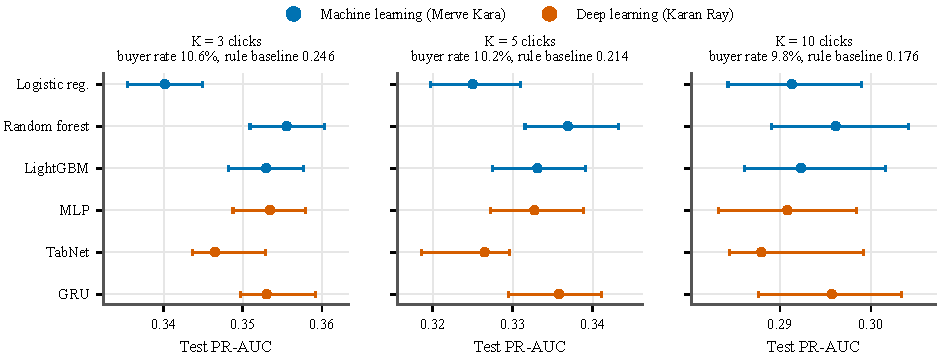
\includegraphics[width=\textwidth]{fig1_rq1_model_comparison.pdf}
  \caption{[Write your caption.]}
  \label{fig:rq1}
\end{figure*}
\begin{table}[t]
\centering
\caption{Test results at $K=5$ (mean $\pm$ sd over seeds 42, 7, 2026); latency per visit, batch size 1.}
\label{tab:main}
\footnotesize
\begin{tabular}{lrrrrrr}
\toprule
Model & PR-AUC & ROC-AUC & F1 & p95 ms & Size MB & Train s \\
\midrule
Rule baseline & 0.2144 $\pm$ 0.0000 & 0.6789 & 0.3953 & 0.001 & <0.01 & <1 \\
Logistic reg. & 0.3250 $\pm$ 0.0000 & 0.7590 & 0.4009 & 0.032 & <0.01 & 1 \\
Random forest & 0.3369 $\pm$ 0.0002 & 0.7623 & 0.4000 & 5.412 & 105.13 & 34 \\
LightGBM & 0.3331 $\pm$ 0.0002 & 0.7615 & 0.3990 & 0.158 & 0.93 & 6 \\
MLP & 0.3327 $\pm$ 0.0001 & 0.7608 & 0.3991 & 0.080 & 0.09 & 55 \\
TabNet & 0.3265 $\pm$ 0.0023 & 0.7577 & 0.3952 & 0.944 & 0.83 & 327 \\
GRU & 0.3358 $\pm$ 0.0006 & 0.7557 & 0.4012 & 0.087 & 0.07 & 249 \\
\bottomrule
\end{tabular}
\end{table}


\subsection{Efficiency}
% \begin{figure}[t]\centering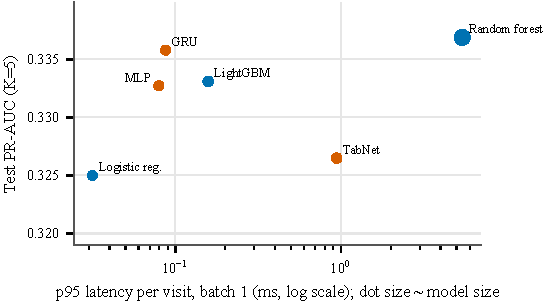
\includegraphics[width=\columnwidth]{fig4_rq4_accuracy_vs_latency.pdf}
% \caption{[Write your caption.]}\label{fig:rq4}\end{figure}

\subsection{Ablation and sensitivity}
% \begin{figure}[t]\centering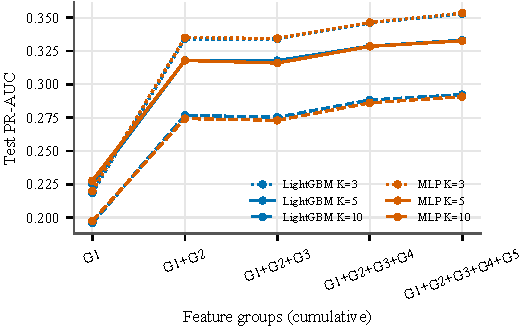
\includegraphics[width=\columnwidth]{fig3_rq3_feature_ladder.pdf}
% \caption{[Write your caption.]}\label{fig:rq3}\end{figure}
\begin{figure}[t]
  \centering
  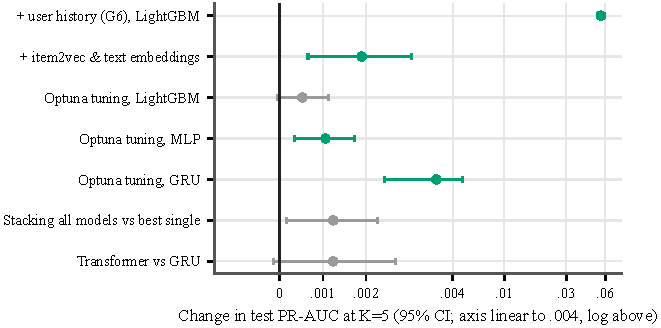
\includegraphics[width=\columnwidth]{fig5_extensions_forest.pdf}
  \caption{[Write your caption.]}
  \label{fig:ext}
\end{figure}

\subsection{Robustness and generalisation}
% \begin{table}[t]
\centering
\caption{Generalisation to all sessions: 10\% sample vs 100\% at $K=5$.}
\label{tab:scale}
\footnotesize
\begin{tabular}{lrrrrr}
\toprule
Model & pr\_auc\_10pct & pr\_auc\_100pct & change & train\_sec\_10pct & train\_sec\_100pct \\
\midrule
GRU & 0.3358 & 0.3371 & 0.0014 & 249 & 1863 \\
Random forest & 0.3369 & 0.3358 & -0.0010 & 34 & 394 \\
LightGBM & 0.3331 & 0.3321 & -0.0010 & 6 & 73 \\
Logistic reg. & 0.3250 & 0.3258 & 0.0008 & 1 & 11 \\
\bottomrule
\end{tabular}
\end{table}

% \begin{figure}[t]\centering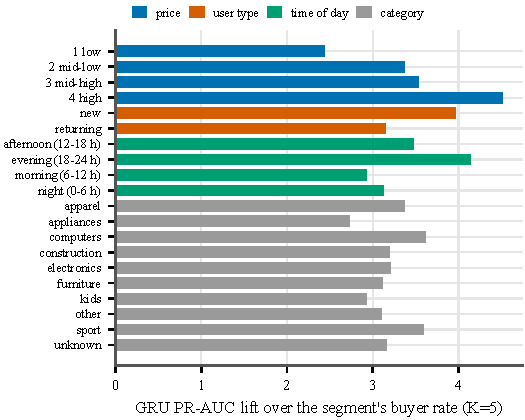
\includegraphics[width=\columnwidth]{fig6_segments_lift.pdf}
% \caption{[Write your caption.]}\label{fig:seg}\end{figure}

\subsection{Error analysis}
% Structured manual analysis from ../error_analysis_sheet.csv (your own categories and counts).

\section{Limitations, Ethics, and Responsible Use}
% ~0.5 page.

\section{Conclusion and Future Work}
% ~0.3 page.

\section*{Reproducibility Statement}
% Code (zip / repository), data access (download script; dataset page as a footnote), environment,
% configuration file, seeds 42/7/2026, procedure (HOW_TO_RUN.md).

\section*{Distribution of Work}
% Who did what (agreed by both authors).

\bibliographystyle{IEEEtran}
\bibliography{../references}

\end{document}
